\documentclass{article}
\usepackage{graphicx}
\usepackage{hyperref}
\usepackage{xcolor}
\usepackage{float}
\usepackage{fancyvrb}
\usepackage{amsmath}
\usepackage{spverbatim}
\usepackage[mathletters]{ucs}
\usepackage[utf8x]{inputenc}

\fvset{tabsize=4}


\graphicspath{ {images/} }
\begin{document}
\pagecolor{white}

\title{%
  First Homework \\
  \large HW1 - Algorithm Design Sapienza}

\author{Giulio Serra 1904089}
\date{December 5, 2020}

\maketitle

\begin{titlepage}
\end{titlepage}

\tableofcontents

\begin{titlepage}
\end{titlepage}

\section{Exercise Number 1 }


\newpage

\section{Exercise Number 2 }

In this problem we want to design a flow network where the maximum flow where it is possible to find a seating arrangement with only good pairs.\\\\Assuming we have a set of investors I=\{i1,i2, ... ij\}, a set of founders F=\{f1,f2, ... fi\} and a list of preferences of the founders by the investors (and vice versa), we can define the "good pairs" as the stable pairs: meaning that in the dinner context, both the investors and the founders seated together don't want to trade place with somebody else.\\
We can rappresent this situation with a bipartite graph G=(V,E) where on the left we have all the nodes rappresenting the investors and on the right we have all the nodes rappresenting the founders, the edges rappresent the interest of each investor to make a conversation with a founder(and vice-versa).Assuming that  {\textbar}I{\textbar} = {\textbar}F{\textbar} = n  

\begin{figure}[h]
		\centering
		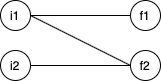
\includegraphics[width=0.2\textwidth ]{EX1-AD.png}
		\caption{Base case where n=2 (since we now that a table must have at least 3 people)}
\end{figure}

Now we have to prove that G has a perfect matching, we can use the Hall's Theorem: Let G = (I {$\cup$} F, E) be a bipartite graph with {\textbar}I{\textbar} =  {\textbar}F{\textbar}. G has a perfect matching if {\textbar}N(S){\textbar} {$\geq$} {\textbar}S{\textbar} for all subsets S {$\subseteq$} F.\\\\And indeed that's true in G, so it must contain a perfect matching.\\\\Now we have to design the bipartite grap G' rappresenting the network flow derived from G, we have to add to nodes: source(s) and sink(t) along with enough edges to connect s and t to both the investors(with s) and the founders(with t), each of those edges will have capacity of 1 while the edges contained in G will have infinite capacity:

\begin{figure}[h]
		\centering
		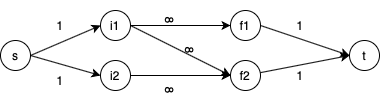
\includegraphics[width=0.6\textwidth ]{DIG_EX1-AD}
\end{figure}

The flow on G' respect both the requirements of capacity and flow conservation. Since G' strictly derive from G (that respect the Hall's theorem) it must exist a maximum flow that is composed by the augmenting paths passing on the edges between I and F that rappresent the stable pairs, therefore we prooved our claim.
 \newpage
 
 \section{Exercise Number 3}
 
Having a set of n projects P, each one having a minimum credit score cp and a reward bp (positive or negative) , we want to find (if it exist) an order in wich a user (starting with a skill score C), can accept all of them in a certain order (also, for each project cp + bp {$\geq$} 0). Here is a solution using a greedy algorithm:
 

 \begin{Verbatim}[fontsize=\small]
	input: set of projects P , user score
	
	S = P sorted by reward from lowest to highest bp1 <= bp2 <=... bpi
	A ← ∅  set of accepted projects
	N ← ∅  set of projects with negative reward 
	
	while S is not empty

		pi = S[i]  i-project of S
		
		if pi reward < 0 
			N = N  ∪ pi
			S = S - {pi}
			
		if pi minimum credit score  <= C
			C += pi reward
			A = A ∪ pi
			S = S - {pi}
		else
			return ∅
		
		i = i + 1
			
	for j = last index of N to 0
		pj = N[j]
		
		if pj minimum credit score  <= C
			C += pj reward
			A = A ∪ pj
		else
			return ∅
		
		j = j - 1
		
	return ∅
			
\end{Verbatim}
\underline{Claim:} The algorithm run in O(nlogn)\\\\\underline{Proof:} The sorting of the project takes O(nlogn), while the two for cycles takes O(2n) in the worst case scenario (all the projects with negative reward), since O(nlogn) goes to infinity faster than O(2n), the algorithm needs at least  O(nlogn) time.\\\\
\underline{Claim:} The algorithm find an optimal solution A if it exist one or return an empty set.\\
\\\underline{Proof:} Suppose that A is not an optimal solution, hence S must contain another project p compatible with the user score C not contained in A, but the greedy algorithm terminates the first cycle by only when S is empty -- a contradiction.

 


\end{document}